\documentclass[hyperref={pdfpagelabels=false}]{beamer}

\usepackage{lmodern}
\usepackage{polski}
\usepackage[utf8]{inputenc}
\usepackage{graphicx}
\usepackage{subfig}
\usetheme{Dresden}
\usecolortheme{beaver}

\author{Piotr Joński}

\title{System zarządzania projektami dedykowany metodyce Scrum}
\institute[Uniwersytet]{
	\inst{}
	Uniwersytet Zielonogórski\\
	\and
	\inst{}
	Wydział Informatyki, Elektrotechniki i Automatyki\\
	\and	
	\inst{}
	Informatyka, Sieciowe Systemy Informatyczne
	\and
	\inst{}
	Promotor dr inż. Andrzej Marciniak
}

\begin{document}
\begin{frame}	
	\titlepage
\end{frame}

\begin{frame}
	\frametitle{Agenda}
	\tableofcontents
\end{frame}

\section{Wstęp}
\begin{frame}
	\frametitle{Wstęp}
	Celem pracy był projekt oraz implementacja systemu do zarządzania projektami.
	System dedykowany jest metody Scrum, która jest jedną z najbardziej popularnych metod wytwarzania oprogramowania.
\end{frame}

\section{Czym jest metodyka Scrum}
\begin{frame}
	\frametitle{Czym jest metodyka Scrum}
Scrum jest zwinną metodyką wytwarzania oprogramowania. 
Jej~początki sięgają lat 80-tych.
Jej główne założenia to:
\begin{itemize}
	\item stały kontakt z klientem
	\item zamiana dokumentacji na implementację
	\item iteracyjne i przyrostowe wytwarzanie oprogramowania (sprint)
	\item jak najszybsze rozwiązywanie konfliktów
	\item codzienne spotkania (stand-up) 
	\item implementacje oparte są o historyjki
\end{itemize}

Wraz ze Scrumem idą w parze inne zwinne metodyki takie: Test Driven Development (TDD) czy Feature Driven Development (FDD).
\end{frame}

\section{Przegląd dostępnych narzędzi}
\begin{frame}
	\frametitle{Przegląd dostępnych narzędzi}
	Obecnie na rynku jest wiele narzędzi, które umożliwiają zarządzanie projektami. Wiele z nich jest dedykowane metodykom zwinnym, a w szczególności Scrumowi.
	\pause
	
	Podstawowymi są:
	\pause
	\begin{itemize}
		\item Jira - darmowa tylko do 10 użytkowników. Posiada wiele rozbudowanych funkcji, które nie są wymagane przez 70\% firm. Jeden z najdroższych systemów.
		\pause
		\item Bitbucket - tylko hosting zewnętrzny. Prywatne repozytoria do 5 osób. Prosty w obsłudze. Uboga funkcjonalność w porównaniu do Jiry.
		\pause
		\item GitHub Issue Tracker - darmowy tylko dla projektów o otwartym kodzie źródłowym. Tylko podstawowa funkcjonalność.
	\end{itemize}
\end{frame}

\section{Cel i zakres pracy}
\begin{frame}
	\frametitle{Cel i zakres pracy}
		Praca w swoim zakresie obejmuje:
		\pause
		\begin{itemize}			
			\item Zapoznanie się z literaturą tematu.
			\pause
			\item Opracowanie założeń projektu.
			\pause
			\item Spis wymagań funkcjonalnych i niefunkcjonalnych systemu.
			\pause
			\item Implementacja wszystkich funkcjonalności.
			\pause
			\item Przetestowanie systemu oraz usunięcie ewentualnych błędów.
		\end{itemize}
\end{frame}
\begin{frame}
	\frametitle{Cel i zakres pracy cd.}
		Natomiast wymagania postawione wytworzonemu systemowi to:
		\pause
		\begin{itemize}
			\item Łatwość instalacji, która została osiągnięta dzięki narzędziu Docker.
			\pause
			\item Przejrzysty interfejs użytkownika, zapewniony przez darmową bibliotekę Primefaces.
			\pause
			\item Brak nadmiarowej funkcjonalności - implementacja tylko obligatoryjnych funkcji tego typu systemu.
		\end{itemize}
\end{frame}

\section{Wybrane założenia i analiza biznesowa}
\begin{frame}
	\frametitle{Wybrane założenia i analiza biznesowa}
	Wytwarzanemu systemowi towarzyszyła metodyka Scrum. Z tego względu wszystkie wymagania funkcjonalne są zapisane w postaci historyjek użytkownika. Historyjki mogą mieć wiele wzorców. \pause W tej pracy stosowane są dwa z nich:
	\pause
	\item Jako \pause \textit{\textless typ użytkownika\textgreater} \pause mogę \pause \textit{\textless nazwa zadania\textgreater}.
	\pause
	\item Jako \textit{\textless typ użytkownika\textgreater} mogę \textit{\textless nazwa zadania\textgreater} \pause w celu \pause \textit{\textless cel\textgreater}.	
\end{frame}
\begin{frame}
	\frametitle{Wybrane założenia i analiza biznesowa cd.}
	Przykładowymi historyjkami użytkownika, które zostaną omówione są:
	\pause
	\begin{itemize}
		\item Jako administrator mogę tworzyć nowych użytkowników w celu dodania ich do systemu.
		\pause
		\item Jako administrator mogę dodawać i usuwać użytkowników z grup w celu modyfikacji zespołu.
	\end{itemize}
\end{frame}
\begin{frame}
	\frametitle{Wybrane założenia i analiza biznesowa cd.}
	\begin{figure}
		\centering
		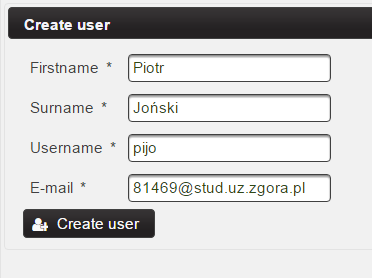
\includegraphics[width=0.7\linewidth]{user-stworz}
	\end{figure}
\end{frame}
\begin{frame}
	\frametitle{Wybrane założenia i analiza biznesowa cd.}
	\begin{figure}
	\centering
	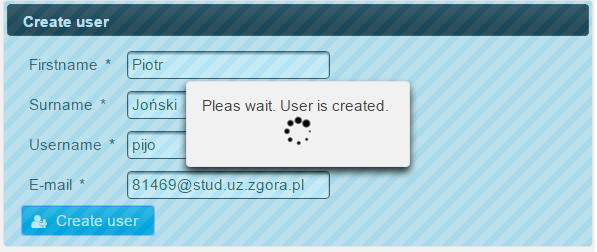
\includegraphics[width=1\linewidth]{user-czekanie}
	\end{figure}
\end{frame}
\begin{frame}
	\frametitle{Wybrane założenia i analiza biznesowa cd.}
	\begin{figure}
		\centering
		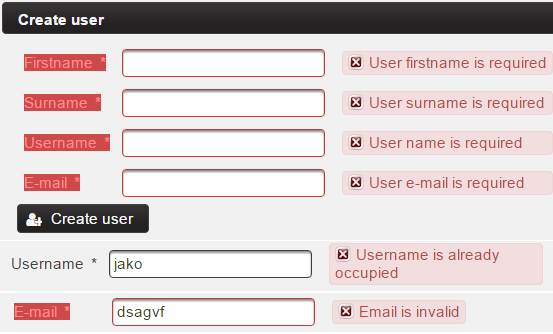
\includegraphics[width=1\linewidth]{user-blad}
	\end{figure}
\end{frame}
\begin{frame}
	\frametitle{Wybrane założenia i analiza biznesowa cd.}
	\begin{figure}
		\centering
		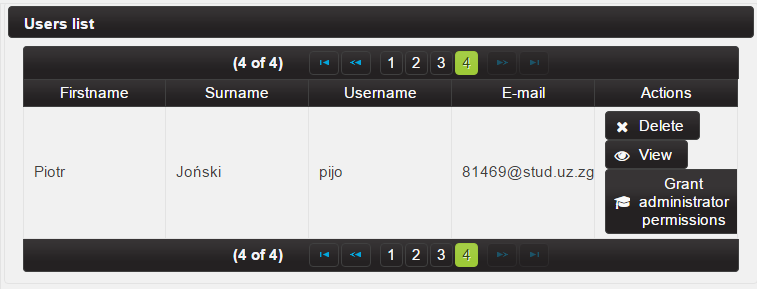
\includegraphics[width=1\linewidth]{user-list}
	\end{figure}
\end{frame}

\begin{frame}
	\frametitle{Wybrane założenia i analiza biznesowa cd.}
	\begin{figure}
		\centering
		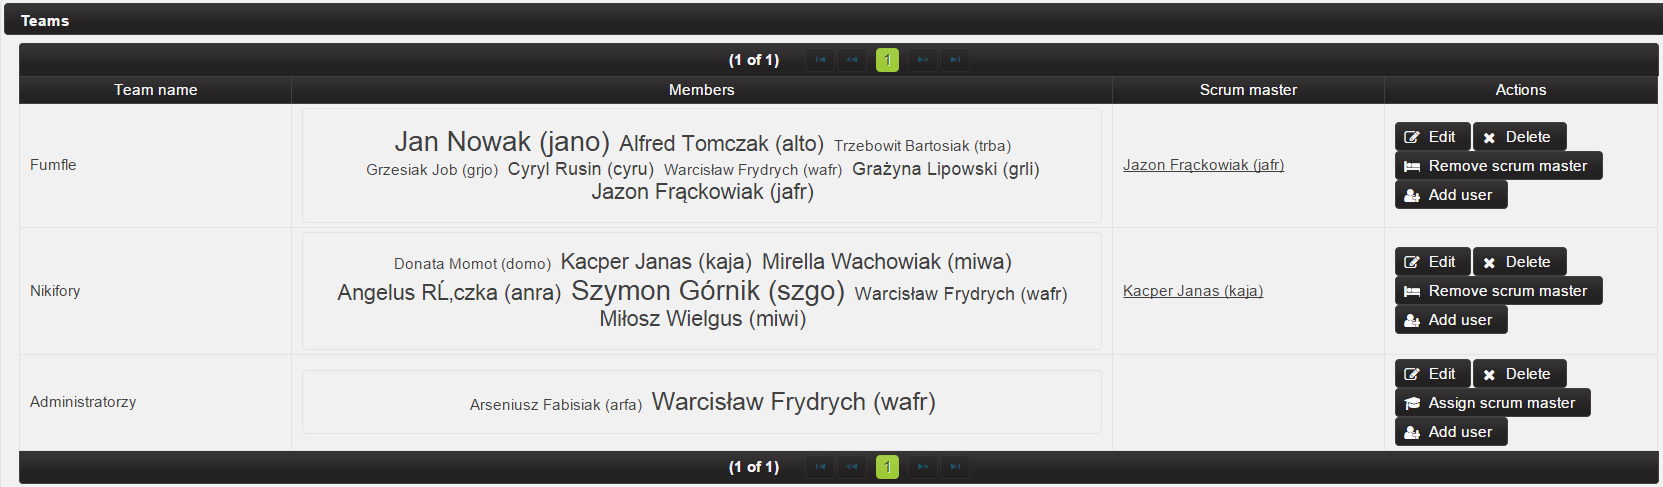
\includegraphics[height=0.5\linewidth, width=1\linewidth]{team-list}
	\end{figure}
\end{frame}
\begin{frame}
	\frametitle{Wybrane założenia i analiza biznesowa cd.}
	\begin{figure}
		\centering
		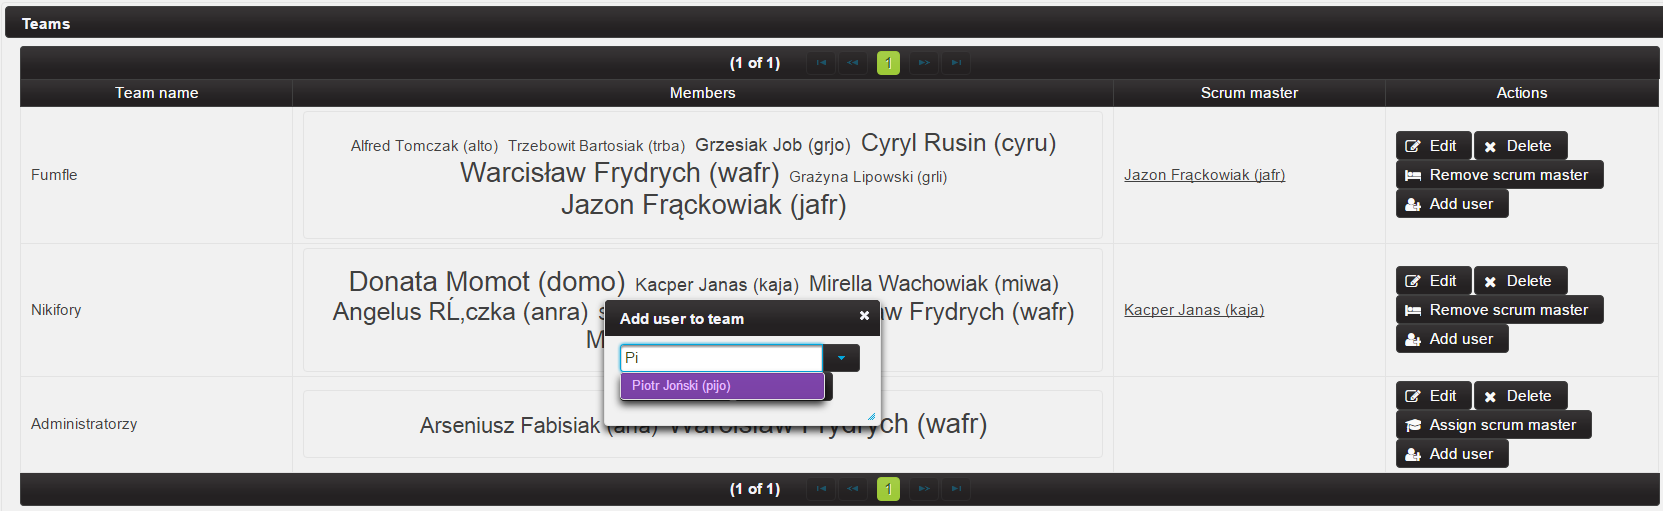
\includegraphics[height=0.5\linewidth, width=1\linewidth]{team-list-add}
	\end{figure}
\end{frame}\begin{frame}
\frametitle{Wybrane założenia i analiza biznesowa cd.}
\begin{figure}
	\centering
	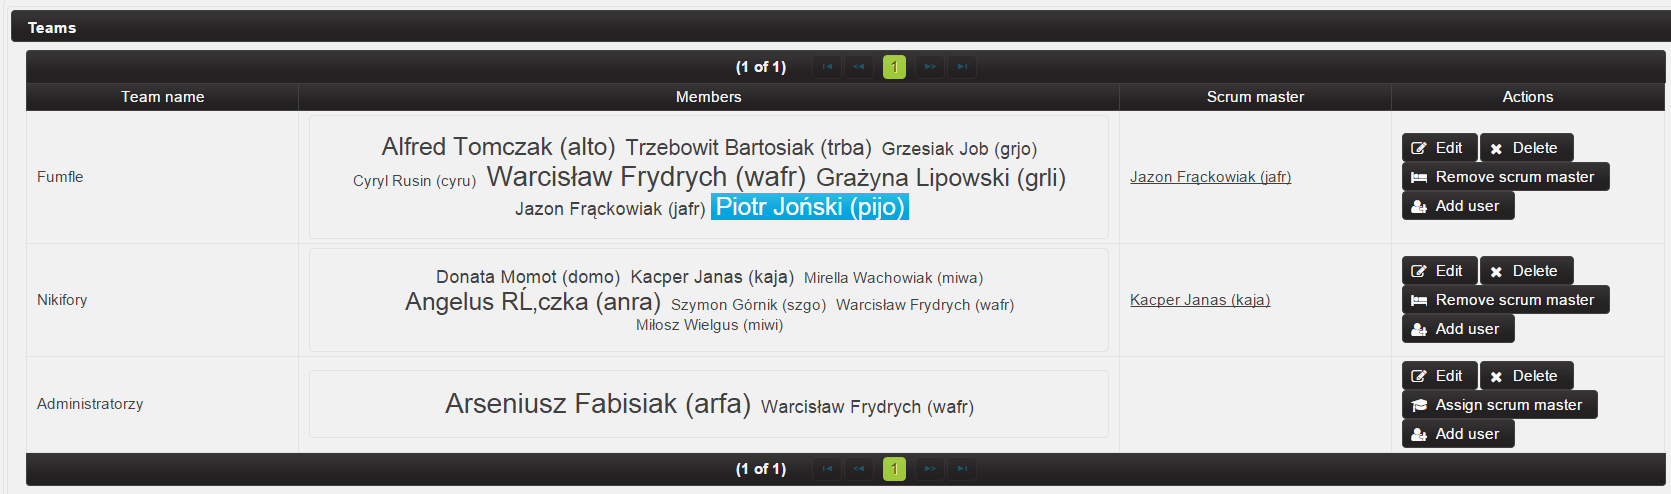
\includegraphics[height=0.5\linewidth, width=1\linewidth]{team-list-del}
\end{figure}
\end{frame}\begin{frame}
\frametitle{Wybrane założenia i analiza biznesowa cd.}
\begin{figure}
	\centering
	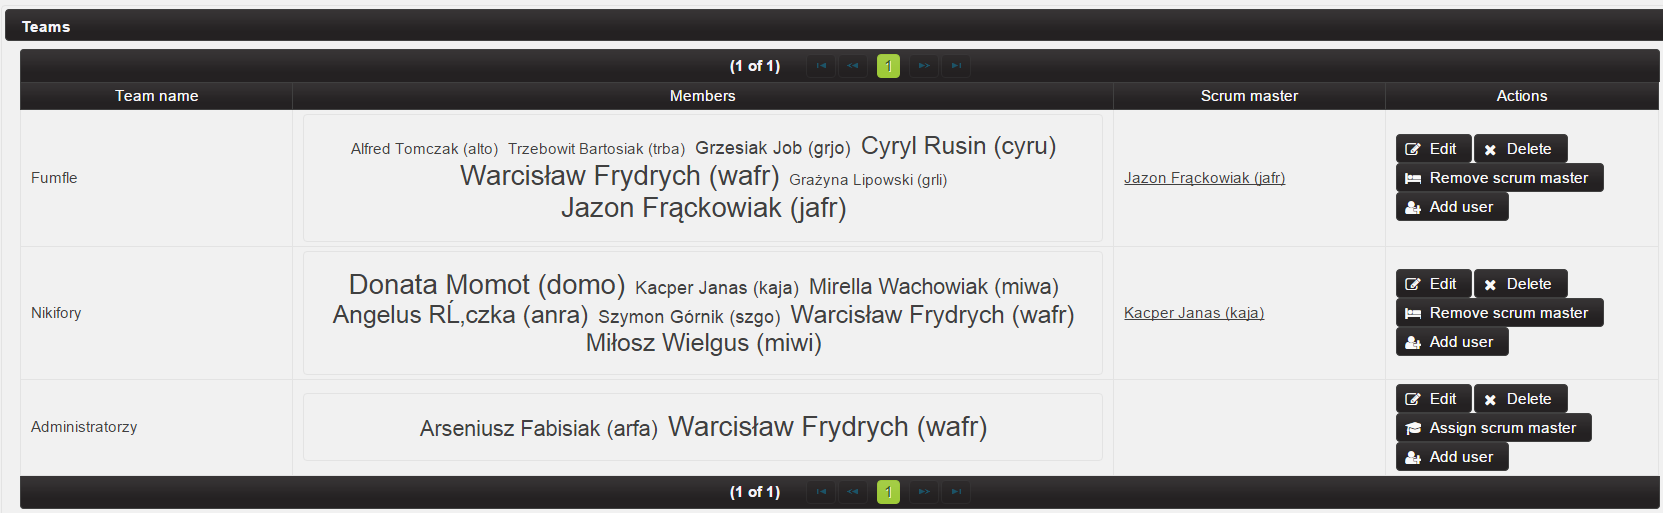
\includegraphics[height=0.5\linewidth, width=1\linewidth]{team-list-del-2}
\end{figure}
\end{frame}

\section{Prezentacja narzędzi}
\begin{frame}
	\frametitle{Prezentacja narzędzi}
\end{frame}

\section{Pytania}
\begin{frame}
	Czas na pytania.
\end{frame}

\end{document}